\section{Results}

The purpose of this thesis work was to design and implement an interactive and semi automated web based tool for discovering association rules from the Carat data that indicate what system settings and usage patterns of a mobile application lead to increased battery consumption. In practise, this has proven to be quite challenging for a number of reasons:

\begin{itemize}
  \item Automatically deciding a sufficient threshold for support and confidence for generating rules is difficult 
  \item Number of generated rules increases rapidly as support and confidence thresholds are lowered
  \item Identifying interesting or relevant rules in presence of hundreds or thousands of rules is cumbersome
  \item Deciding how to discretize ordinal and continuous variables is non-trivial          
\end{itemize}

We will now look at the results of this work in two parts. In the first part we will be looking at the performance of the application and how it affects its usability. In the second part we will take a look at some example use cases of the system.  

\subsection{Performance Evaluation}

\begin{figure}[htp]

\subfloat[Number of rules with fitted plane]{
  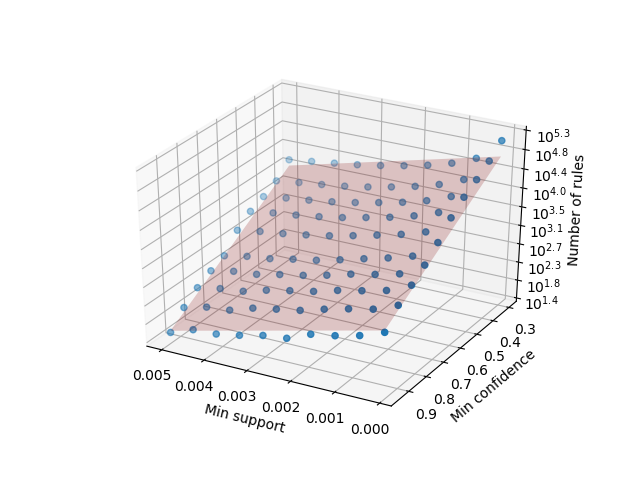
\includegraphics[width=\textwidth]{images/results/facebook_num_rules.png}%
}

\subfloat[Number of rules with error bars]{%
  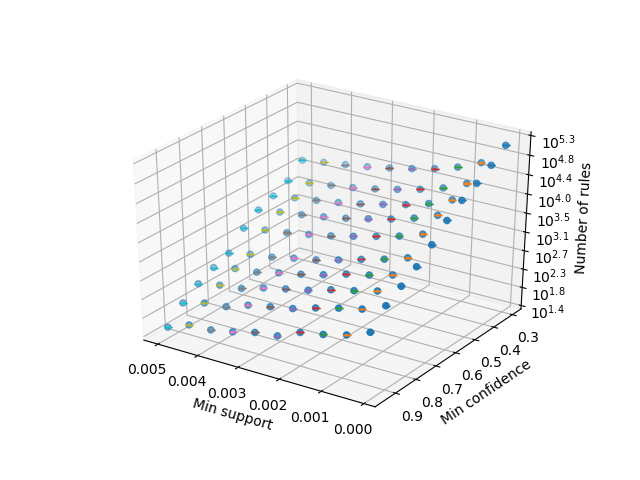
\includegraphics[width=\textwidth]{images/results/facebook_num_rules_with_error_bars.png}%
}

\caption{Number of generated rules for Facebook measurements as a function of minimum support threshold and minimum confidence threshold}
\label{figure:number-of-rules-facebook}
\end{figure}

In order to understand the relationship between the number of generated rules and minimum support and confidence thresholds, a series of measurements were conducted on the Carat API prototype server. Figure~\ref{figure:number-of-rules-facebook} shows these  measurements for Facebook application and Figure~\ref{figure:number-of-rules-spotify} shows the measurements for Spotify application. The figures show the relationship of generated rules as a function of minimum support threshold and confidence threshold as a three dimensional plot. A series of five measurements were conducted for each application. In each of series, a minimum confidence threshold range of 0.3 to 0.9 and a minimum support threshold range of 0.0001 to 0.005 were both divided evenly by 10 points creating a grid of 100 points where the measurements were taken. The blue dots represent average of the five measurement at each point of the support-confidence-grid. In sub figure A, a plane was fitted to the measurements points using least squares method. This was done to better illustrate the spatial configuration of the measurements as well as to showcase how well the measured points are aligned on the plane. In sub figure B, error bars were plotted to the measurements using one standard deviation of the five measurements as the size of the error. 

%Figure~\ref{figure:number-of-ruless} shows the relationship of these variables on two selected applications, namely Spotify and Facebook mobile applications. The blue dots represent individual measurements. A minimum confidence threshold range of 0.3 to 0.9 and a minimum support threshold range of 0.0001 to 0.005 were both divided evenly by 10 points creating a grid of 100 points where the measurements were taken. The number of rules -axis is in $log_{10}$ scale to better illustrate the varying magnitudes of the number of generated rules. The transparent red plane was fitted to the measured points using the least squares method.

The number generated rules seems to grow exponentially on both axes when approaching zero, as can be seen by how well the measurements align with the least squares plane. This explosion in the number of generated rules makes it difficult for the user to extract useful rules from the system when small values for the thresholds are used. To mitigate this problem, the system provides two features:

\begin{itemize}
	\item The generated rules are sorted in the ascending order of their confidence, giving the more reliable rules a greater priority.    
         
	\item Attributes can be excluded from the analysis - potentially greatly reducing the number of generated rules. 
\end{itemize}        

Even though there is a stochastic component in the rule generation, which arises from the sampling of data in the variable discretization stage of the analysis, the number of generated rules does not seem to vary much, as can be seen from the error bars, which are barely visible.  


\begin{figure}[htp]
\subfloat[Number of rules with fitted plane]{
  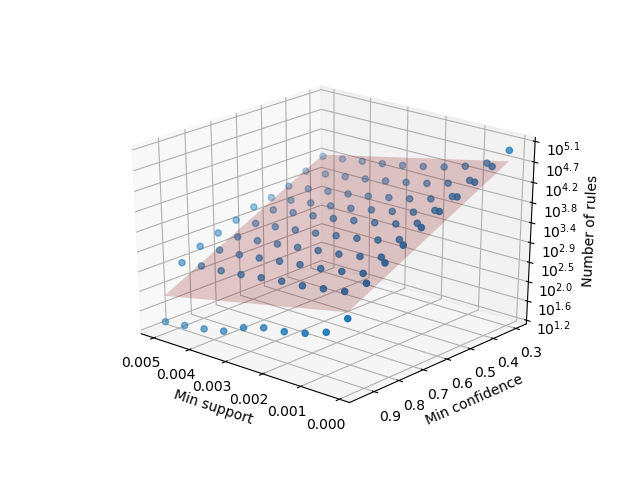
\includegraphics[width=\textwidth]{images/results/spotify_num_rules.png}%
}

\subfloat[Number of rules with error bars]{%
  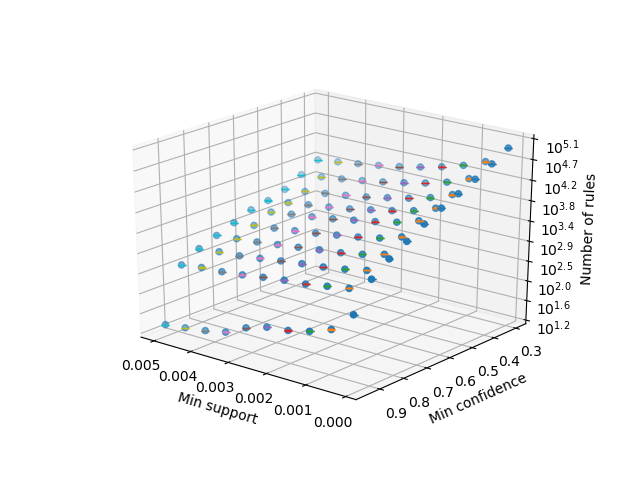
\includegraphics[width=\textwidth]{images/results/spotify_num_rules_with_error_bars.png}%
}

\caption{Number of generated rules for Spotify measurements as a function of minimum support threshold and minimum confidence threshold}
\label{figure:number-of-rules-spotify}
\end{figure}


%\begin{figure}[htp]
%\subfloat[Facebook mobile application]{%
%  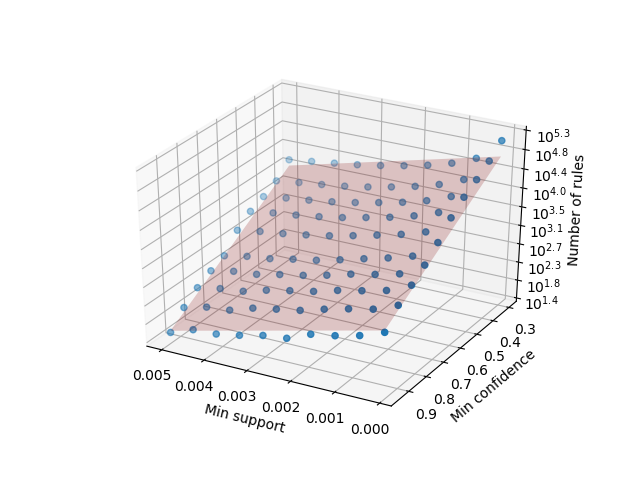
\includegraphics[width=\textwidth]{images/results/facebook_num_rules.png}%
%}
%\subfloat[Spotify mobile application]{%
%  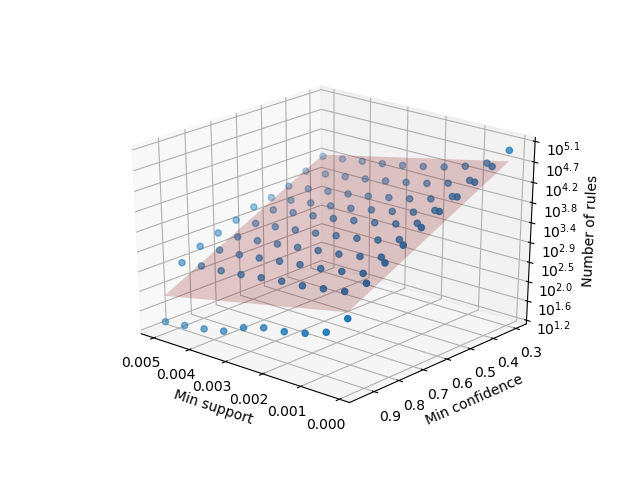
\includegraphics[width=\textwidth]{images/results/spotify_num_rules.png}%
%}
%\caption{Number of generated rules plotted as a function of minimum support threshold and minimum confidence threshold}
%\label{figure:number-of-ruless}
%\end{figure}

\begin{figure}[htp]

\subfloat[Rule generation time with best fitting plane]{
  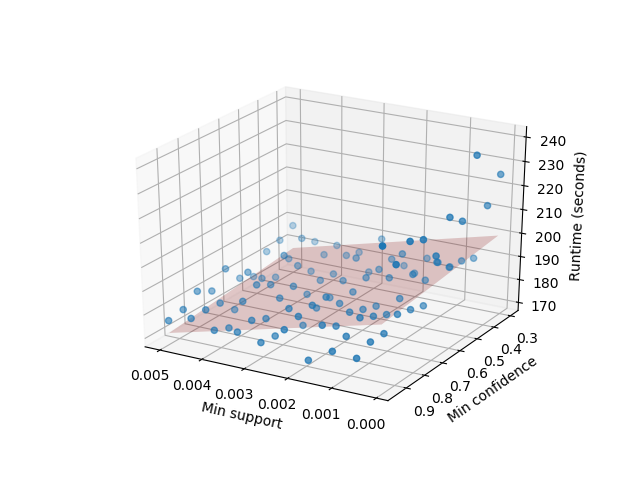
\includegraphics[width=\textwidth]{images/results/facebook_runtimes.png}%
}

\subfloat[Rule generation time with error bars]{%
  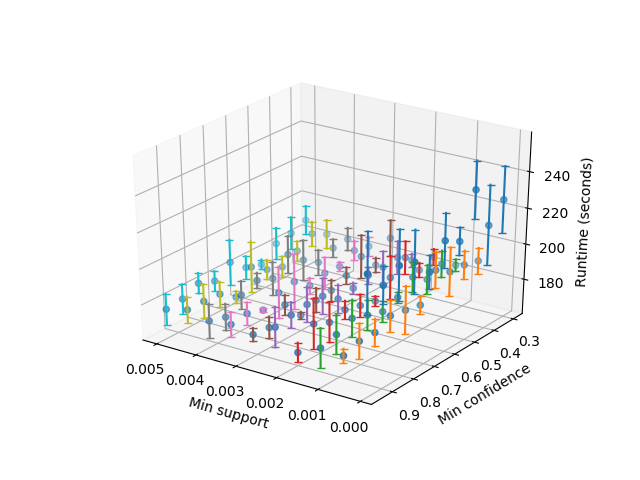
\includegraphics[width=\textwidth]{images/results/facebook_runtimes_with_error_bars.png}%
}

\caption{Rule generation time for Facebook measurements as a function of minimum support threshold and minimum confidence threshold}
\label{figure:runtimes-facebook}
\end{figure}

In addition to the number of generated rules, another metric that is a good indicator for usability of the system, is the time taken to generate the association rules. To measure the time of the rule generation as a function of minimum support threshold and minimum confidence threshold, a similar set up as with the number of generated rules was used. Figure~\ref{figure:runtimes-facebook} shows these measurements for the Facebook application and Figure~\ref{figure:runtimes-spotify} shows the measurements for the Spotify application. Like before, the blue dots represent the average value in five measurements series of 100 measurement points. The red plane represents a plane that was fitted to the points using the least squares method. The size of the error in the error bars is again the standard deviation of the measurement at each measurement point.

The rule generation time increases as either axis approaches zero. The deviance is not huge however, as all the measured run times fall between 160 and 260 seconds. While this is a notable difference from the users perspective, the system remains usable even when the number of generated rules is in the order of $10^5$.   

\begin{figure}[htp]

\subfloat[Rule generation time with best fitting plane]{
  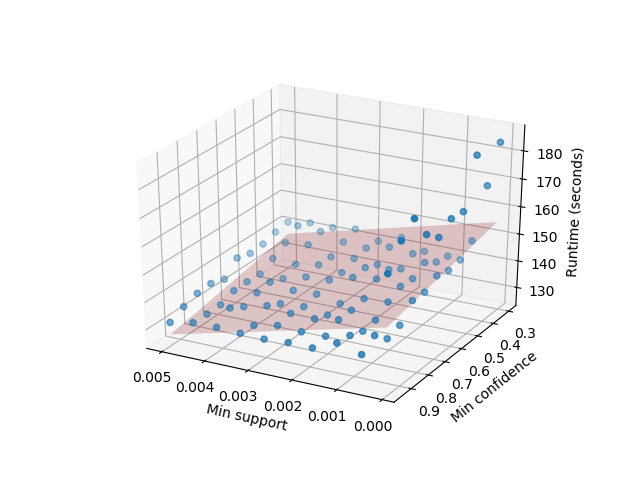
\includegraphics[width=\textwidth]{images/results/spotify_runtimes.png}%
}

\subfloat[Rule generation time with error bars]{%
  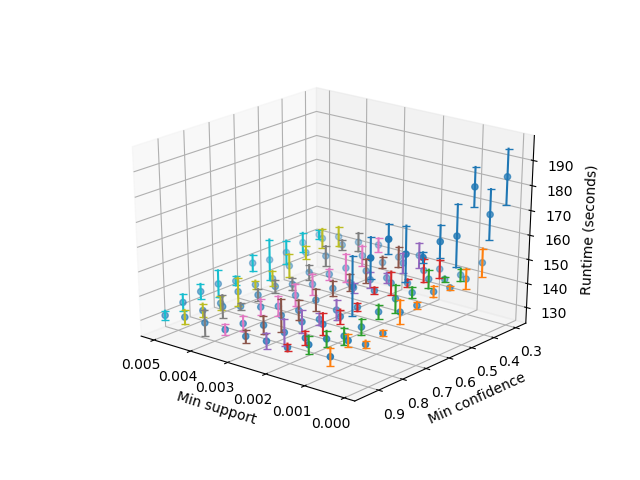
\includegraphics[width=\textwidth]{images/results/spotify_runtimes_with_error_bars.png}%
}

\caption{Rule generation time for Spotify measurements as a function of minimum support threshold and minimum confidence threshold}
\label{figure:runtimes-spotify}
\end{figure}

All the experiments were conducted on a Spark cluster which had a single computing server. For each run, 45 CPU cores and 1500 gigabytes of memory were reserved. To mitigate the effect of any potential file server load, the dataset was stored in memory using Linux shared memory file system (/dev/shm). The dataset consisted of Carat samples from 22.6.2016 to 22.8.2016, the size of which was a little over 16 gigabytes.


%\begin{figure}[htp]
%\subfloat[Facebook mobile application]{%
%  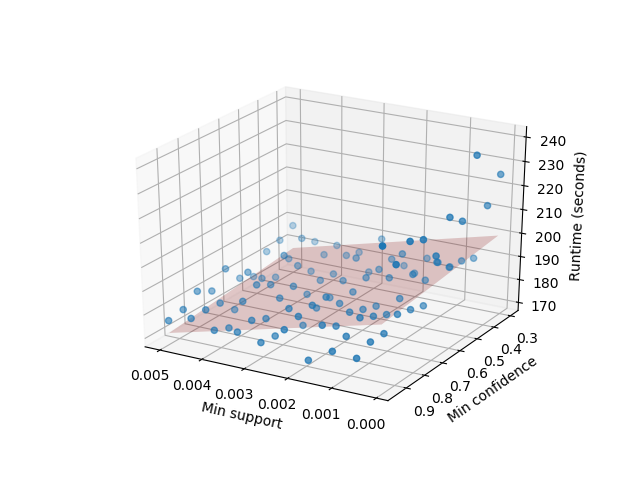
\includegraphics[width=\textwidth]{images/results/facebook_runtimes.png}%
%}
%\subfloat[Spotify mobile application]{%
%  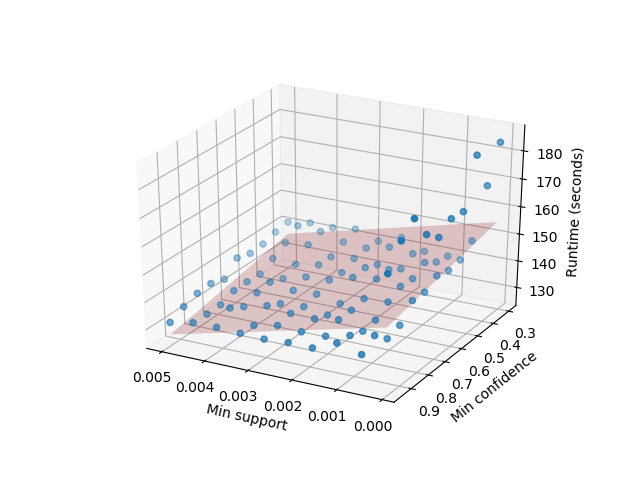
\includegraphics[width=\textwidth]{images/results/spotify_runtimes.png}%
%}
%\caption{Association rule generation time as a function of minimum support threshold and minimum confidence threshold}
%\label{figure:analysis-runtime}
%\end{figure}  

\subsection{Overview on Generated Rules}

For this section, four popular Android applications were selected to be inspected with the rule generation. The selected applications were com.facebook.katana, com.google.android.chrome, com.google.android.apps.photos and com.spotify.music. To achieve comparable results, the minimum support threshold was fixed to 0.001 and the minimum confidence threshold was fixed to 0.5. Given that the least popular of these applications in the dataset used for this analysis contained little over 420 000 data points, a minimum support threshold of 0.001 means that for each generated rule, there should always be at least 420 data points supporting that rule. For each of these four applications, a total of six of the generated rules were selected for further inspection. These six rules were selected by taking the three most confident rules that predicted high energy consumption rate and the three most confident rules that predicted low energy consumption rate.  

Table~\ref{table:rules-facebook} shows the generated rules for the com.facebook.katana mobile application. Looking at the top three rules that predicted hight energy rate for the application, it seems that using HSDPA type mobile network connection and a high screen brightness were clearly connected to high energy consumption. When these two factors were combined with high battery temperature, we get the most confident of these three rules with a confidence score of 0.5811. As the highest confidence rule in this category had a confidence score of less than 0.6, one can say that there were no clear explanations of high energy consumption to be found by these variables for this particular application. Looking at the three most confident rules for low energy consumption, the common factors seem to be using WiFi connection, low battery temperature and low or medium low CPU usage. Notably, the rules for low energy consumption had significantly greater confidence than the rules for high energy consumption. The highest confidence for these three rules was 0.9985 while the lowest was 0.9964. 

\begin{table} \small%
\begin{tabular}{|p{5.0cm}|p{3.0cm}|p{2.0cm}|p{1.5cm}|p{0.3cm}| p{0.3cm}|}
\hline
Antecedents & Consequent & Confidence \\
\hline
	mobileNetType=hsdpa 		& & \\
	screen is 222 - 255			& rate is 0.011 - 1.0 & 0.5811 \\
	temperature is 35 - 88		& & \\
\hline
	mobileNetType=hsdpa			& & \\
	screen is 222 - 255			& & \\
	cpu is 0.39 - 0.62			& rate is 0.011 - 1.0 & 0.5464 \\
	voltage is 0 - 3			& & \\
	distance=no					& & \\
\hline
	mobileNetType=hsdpa			& & \\
	screen is 222 - 255			& rate is 0.011 - 1.0 & 0.5432 \\
	cpu is 0.39 - 0.62			& & \\
	voltage is 0 - 3			& & \\
\hline
	mobileNetType=unknown		& & \\
	screen is 222 - 255			& & \\
	wifiStrength is -99 - -69	& rate is 0.0 - 0.00017 & 0.9985 \\
	cpu is 0.0 - 0.39			& & \\
	temperature is 5 - 28		& & \\
	voltage is 3 - 4			& & \\
\hline
	mobileNetType=unknown		& & \\
	screen is 222 - 255			& & \\
	wifiStrength is -99 - -69	& rate is 0.0 - 0.00017 & 0.9974 \\
	wifiSpeed is 54 - 72		& & \\
	cpu is 0.39 - 0.62			& & \\
	temperature is 5 - 28		& & \\
	voltage is 0 - 3			& & \\
\hline
	mobileNetType=unknown		& & \\
	screen is 222 - 255			& & \\
	wifiSpeed is 0 - 54			& rate is 0.0 - 0.00017 & 0.9964 \\
	cpu is 0.39 - 0.62			& & \\
	temperature is 5 - 28		& & \\
	voltage is 3 - 4			& & \\
\hline
\end{tabular}
	\caption{Selected rules for the com.facebook.katana mobile application}
	\label{table:rules-facebook}
\end{table}

In Table~\ref{table:rules-android-photos} shows the selected rules for the com.google.android.apps.photos application. In this case, the factors that indicated high energy consumption were using GPRS for mobile networking, having weak WiFi singnal strength and low WiFi signal speed and low battery voltage. The low battery voltage may indicate a certain set of mobile devices that perform poorly when the other factors are also present. The confidence of these rules were reasonable, ranging from 0.7100 to 0.7074. The most confident rules for low energy consumption all had the common factors of using UTMS mobile network connection, high WiFi link speed, medium low CPU usage and weirdly enough, high screen brightness. 

\begin{table} \small%
\begin{tabular}{|p{5.0cm}|p{3.0cm}|p{2.0cm}|p{1.5cm}|p{0.3cm}| p{0.3cm}|}
\hline
Antecedents & Consequent & Confidence \\
\hline
	mobileNetType=gprs				& & \\
	wifiStrength is -100 - -68		& & \\
	wifiSpeed is 0 - 54				& & \\
	netType=wifi					& rate is 0.011 - 1.0 & 0.7100 \\
	voltage is 0 - 3				& & \\
	distance=no						& & \\
\hline
	mobileNetType=gprs				& & \\
	wifiStrength is -100 - -68		& & \\
	wifiSpeed is 0 - 54				&  rate is 0.011 - 1.0 & 0.7082 \\
	voltage is 0 - 3				& & \\
	distance=no						& & \\
\hline
	mobileNetType=gprs				& & \\
	wifiStrength is -100 - -68		& & \\
	wifiSpeed is 0 - 54				& rate is 0.011 - 1.0 & 0.7074 \\
	netType=wifi					& & \\
	voltage is 0 - 3				& & \\
\hline
	screen is 220 - 255				& & \\
	mobileNetType=utms				& & \\
	wifiSpeed is 144 - 6477		& rate is 0.0 - 0.0015 & 0.9966 \\
	wifiStrength is -68 - -59		& & \\
	cpu is 0.42 - 0.67				& & \\
\hline
	screen is 220 - 255				& & \\
	mobileNetType=utms				& & \\
	wifiSpeed is 144 - 6477		& rate is 0.0 - 0.0015 & 0.9965 \\
	wifiStrength is -68 - -59		& & \\
	cpu is 0.42 - 0.67				& & \\
	voltage is 3 - 4				& & \\
\hline
	screen is 220 - 255				& & \\
	mobileNetType=utms				& & \\
	wifiSpeed is 144 - 6477		& rate is 0.0 - 0.0015 & 0.9936 \\
	cpu is 0.42 - 0.67				& & \\
	voltage is 3 - 4				& & \\
\hline
\end{tabular}
	\caption{Selected rules for the com.google.android.apps.photos mobile application}
	\label{table:rules-android-photos}
\end{table}

Table~\ref{table:rules-chrome} shows the selected rules for the com.android.chrome mobile application. There were no rules, within the given confidence constraint, that predicted an energy consumption rate in the highest quantile, so instead the three top rules in the table are the three highest confidence rules that predicted an energy consumption rate in the third quantile within the samples where the Chrome application was running. Within the rules which predicted high energy consumption, common factors were high screen brightness, high battery temperature, fast WiFi link speed and using LTE type mobile networking. The confidence of these rules ranged from 0.6519 to 0.65. Looking at the rules which predicted low energy consumption, common factors were low battery temperature, fast WiFI link speed, mobile networking type UTMS and again, oddly enough, a high screen brightness. The confidence of the rules predicting low energy consumption were again very high, ranging from 0.9985 to 0.9964.   

\begin{table} \small%
\begin{tabular}{|p{5.0cm}|p{3.0cm}|p{2.0cm}|p{1.5cm}|p{0.3cm}| p{0.3cm}|}
\hline
Antecedents & Consequent & Confidence \\
\hline
	screen is 206 - 255 			& & \\
	wifiSpeed is 135 - 4728		& & \\ 
	temperature is 34 - 88  		& rate is 0.0046 - 0.011 &  0.6519 \\
	mobileNetType=lte				& & \\
	netType=wifi					& & \\
\hline
	screen is 206 - 255				& & \\
	wifiSpeed is 135 - 4728 		& rate is 0.0046 - 0.011 & 0.6506 \\
	temperature is 34 - 88			& & \\
	mobileNetType=lte				& & \\
\hline
	screen is 206 - 255				& & \\
	wifiSpeed is 135 - 4728 		& & \\
	temperature is 34 - 88			& rate is 0.0046 - 0.011  & 0.65 \\
	mobileNetType=lte				& & \\
	netType=wifi					& & \\
	distance=no						& & \\
\hline
	screen is 206 - 255				& & \\
	mobileNetType=utms				& & \\
	wifiSpeed is 135 - 4728		& rate is 0.0 - 0.0015 & 0.9893 \\
	wifiStrength is -68 - -59		& & \\
	voltage is 3 - 4				& & \\
\hline
	screen is 206 - 255				& & \\
	mobileNetType=utms				& & \\
	wifiSpeed is 135 - 4728		& rate is 0.0 - 0.0015 & 0.9822 \\
	temperature is 5 - 28			& & \\
	voltage is 3 - 4				& & \\
\hline
	screen is 206 - 255				& & \\
	mobileNetType=utms				& rate is 0.0 - 0.0015 & 0.9749 \\
	wifiSpeed is 135 - 4728		& & \\
	temperature is 5 - 28			& & \\
\hline
\end{tabular}
	\caption{Selected rules for the com.google.android.chrome mobile application}
	\label{table:rules-chrome}
\end{table}

In Table~\ref{table:rules-spotify} are listed the selected rules for the com.spotify.music mobile application. In the context of the rules that predict high energy consumption, factors high screen brightness, high WiFi link speed, quite low wiFi signal strength, medium high battery temperature and medium high CPU usage are all shared. Two out of three of these rules also share the factor mobile networking type LTE and low battery voltage. The confidence of these rules ranged from 0.8852 to 0.8821, which compared to the other application's high energy rules, seems very high. Among the rules that predicted low energy consumption, shared factors were mobile networking type UTMS, a medium high CPU usage, and a medium low wiFi signal strength. Factors that were shared by two out of the three rules included high screen brightness, low battery temperature and high WiFi link speed. The confidence score of all three of these rules was 1.0. 

\begin{table} \small%
\begin{tabular}{|p{5.0cm}|p{3.0cm}|p{2.0cm}|p{1.5cm}|p{0.3cm}| p{0.3cm}|}
\hline
Antecedents & Consequent & Confidence \\
\hline
	screen is 210 - 255 		& & \\
	wifiSpeed is 144 - 866		& & \\
	wifiStrength is -68 - -59	& & \\
	temperature is 34 - 60		& rate is 0.012 - 1.0 & 0.8852 \\
	cpu is 0.61 - 0.84			& & \\
	mobileNetType=lte			& & \\
	voltage is 0 - 3			& & \\
\hline
	screen is 210 - 255			& & \\
	wifiSpeed is 144 - 866		& & \\
	wifiStrength is -68 - -59	& rate is 0.012 - 1.0 & 0.8821 \\
	temperature is 34 - 60		& & \\
	cpu is 0.61 - 0.84			& & \\
	voltage is 0 - 3			& & \\
\hline
	screen is 210 - 255			& & \\
	wifiSpeed is 144 - 866		& & \\
	wifiStrength is -68 - -59	& rate is 0.012 - 1.0 & 0.8821 \\
	temperature is 34 - 60		& & \\
	cpu is 0.61 - 0.84			& & \\
	mobileNetType=lte			& & \\
\hline
	mobileNetType=utms			& & \\
	wifiSpeed is 144 - 866		& & \\
	wifiStrength is -68 - -59	& rate is 0.0 - 0.0016 & 1.0 \\
	cpu is 0.61 - 0.84			& & \\
	temperature is 12 - 28		& & \\
	voltage is 3 - 4			& & \\
\hline
	screen is 210 - 255			& & \\
	mobileNetType=utms			& & \\
	wifiStrength is -68 - -59	& rate is 0.0 - 0.0016 & 1.0 \\
	cpu is 0.61 - 0.84			& & \\
	temperature is 12 - 28		& & \\
\hline
	screen is 210 - 255			& & \\
	mobileNetType=utms			& & \\
	wifiSpeed is 144 - 866		& rate is 0.0 - 0.0016 & 1.0 \\
	wifiStrength is -68 - -59	& & \\
	cpu is 0.61 - 0.84			& & \\
\hline
\end{tabular}
	\caption{Selected rules for the com.spotify.music mobile application}
	\label{table:rules-spotify}
\end{table}

The generated example rules are generally not very intuitive and some of the relations, such as the contribution of high screen brightness to low energy consumption, are outright counter intuitive. On the bright side, the system is able to find rules with very high confidence even with a reasonably high support threshold of 0.001. The choice of application also seems to have a reasonable impact on the generated rules, which is promising for the usability of the system. Perhaps interesting is the fact that more confident rules seem to be generated for the low energy consumption than for the high energy consumption. Even if the system is not able to predict with any reasonable accuracy which factors lead to large levels of energy consumption when using a certain application, it might be useful to be able predict with acceptable accuracy which combinations of factors lead to low levels of energy consumption. At the very least, this kind of prediction could be a valuable addition to a recommendation system like the one described in~\cite{PELTONEN201671}.     